\documentclass{article}

\usepackage{amsmath,amsthm}     
\usepackage{graphicx}     
\usepackage{hyperref} 
\usepackage{url}
\usepackage{amsfonts} 
\usepackage[margin=1in]{geometry}
\usepackage{float}
\usepackage{multicol, multirow}
\usepackage{arydshln}
\usepackage{subcaption}
\usepackage[french]{babel}
\usepackage{adjustbox}



\allowdisplaybreaks

\makeatletter
\@addtoreset{footnote}{page}
\makeatother

%%%%%%%%%%%%%%%%%%%%%%%%%%%%%%%%%%%%%%%%%%%%%%%%%%
\begin{document}

\renewcommand{\arraystretch}{1.5}

\title{BIML NLP : Classification d'émotions \\
\footnotesize{}}
\author{Bonhoure Timothé, Martinez Christophe}                      %%%% your final manuscript.

\maketitle
\tableofcontents
\section*{Abstract}
\newpage

\section{Modèle}
Notre architecture de modèle suit fidèlement les spécifications du sujet (voir Figure \ref{fig:modele_rnn}). Le processus commence par l'encodage en One Hot d'un mot en entrée, suivi d'un passage à travers une couche linéaire d'embedding. Par la suite, le modèle concatène la sortie de cette couche d'embedding avec des données cachées internes au modèle, permettant ainsi la mémorisation des mots précédents dans la phrase. Enfin, ces données sont traitées par deux couches en parallèle pour produire en sortie une classification de l'émotion associée à la phrase. De manière récurrente, les informations résultantes sont également réinjectées dans les données cachées pour le traitement du mot suivant. \\
Toutes les couches sont des couches linéaires dont nous initialisons les poids avec la méthode\\ \texttt{nn.init.xavier\_uniform\_} permettant d'après nos recherches d'atténuer les effets de vanishing et d'exploding du gradient.

\begin{figure}[H]
    \centering
    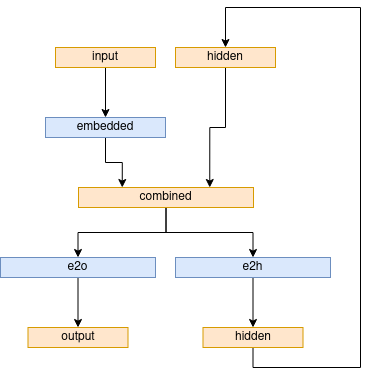
\includegraphics[width=0.4\linewidth]{img/modele.png}
    \caption{Modèle RNN}

    \label{fig:modele_rnn}
\end{figure}

\section{Entrainement}
La tâche principale de notre modèle consiste à classifier l'émotion associée à une phrase donnée. Pour entrainer notre modèle, nous avons choisi d'utiliser la fonction de perte \texttt{CrossEntropyLoss}. Cette fonction est largement adoptée dans les tâches de classification, en raison de sa capacité à inciter le modèle à être plus confiant dans ses prédictions. En effet, \texttt{CrossEntropyLoss} pénalise plus sévèrement les prédictions incorrectes associées à une forte confiance du modèle, favorisant ainsi une meilleure calibration des probabilités prédites. \\
Pour optimiser notre modèle, nous avons opté pour l'utilisation de l'optimiseur \texttt{AdamW}. Cette variante améliorée de l'optimiseur \texttt{Adam} intègre une correction spécifique pour la régularisation des poids, résolvant ainsi le problème de dégradation du poids associé à l'optimiseur \texttt{Adam} standard. \\
Lors de nos tests, nous avons observé une stabilisation de l'apprentissage au cours des 10 à 15 premières époques. Ainsi, choisir 20 époques pour réaliser l'entraînement complet de notre modèle nous est apparu comme un compromis judicieux entre la rapidité et la performance de l'apprentissage. En ce qui concerne la taille du lot (\textit{batch size}), notre approche a été de la laisser non fixée et dépendante du cas de test spécifique. Nous avons adopté cette flexibilité pour nous adapter aux différentes situations d'expérimentation et ainsi évaluer la performance du modèle dans des contextes variés dans des temps comparables.

\section{Préparation des données}
Nous avons décidé de ne conserver que les mots dont la fréquence d’apparition est de minimum 4. Nous estimons que cela équivaut à retirer environ 75\% des mots totaux de notre jeu de données en comptant les doublons. L’effet de ce filtrage a pour effet d’accélérer grandement l’entrainement de notre modèle. \\
En analysant la distribution des longueurs de phrases dans notre ensemble d'entraînement, nous constatons une longueur moyenne d'environ 20 mots avec une variance de 120. Ces statistiques guident notre choix de définir une longueur maximale de phrases à 15 mots pour notre modèle. \\
En plus de cela, nous recourons à la vectorisation TF-IDF pour chercher à extraire les caractéristiques de nos phrases en cherchant les mots les plus importants et significatifs. Parmi les 15 mots conservés de chaque phrase, nous avons préservé ceux présentant un meilleur score selon TF-IDF. \\
Ainsi préparé, notre jeu de données est prêt à être utilisé dans l'entraînement de notre modèle de classification d'émotions. Cette préparation tient compte de la fréquence des mots, de la longueur des phrases, et des caractéristiques TF-IDF significatives, pour tendre au maximum vers une représentation riche et pertinente pour la classification.

\section{Tâche secondaire}
Une couche supplémentaire a été incorporée en parallèle (voir Figure \ref{fig:modele_rnn_with_secondary}) avec les deux précédentes pour accomplir une seconde tâche d'apprentissage basée sur la détection de la négation dans la phrase à classifier. Dans le cadre d'un prétraitement initial, les phrases ont été étiquetées comme étant négatives ou positives. Nous avons établi une liste de mots que nous considérons comme des indicateurs explicites de négation, notamment "not", "never", "neither", "no", "none", "nobody", "nowhere", et "nothing". Ainsi, toute phrase contenant au moins l'un de ces mots est étiquetée comme négative pour l'apprentissage de notre modèle. Pour la marque de négation en anglais "n't", la tâche d'étiquetage a été plus complexe. Pour des raisons de compatibilité des données, les apostrophes de "n't" ont été supprimées ("nt") et/ou remplacées par un caractère espace ("n t"). Ainsi, nous avons ajouté à la liste des indicateurs de négation le mot "t", mais il n'était malheureusement pas possible d'inclure tous les mots finissant par "nt" car cela englobe aussi des mots tels que "comment" et "radiant" qui ne sont pas des marqueurs de négation. Nous avons alors ajouté les mots "dont", "didnt", et "cant" qui sont les marqueurs suivant ce schéma les plus fréquents dans le jeu d'entraînement (entre 250 et 500 occurences).  \\
La tâche du modèle consiste désormais à prédire simultanément l'émotion associée à la phrase et à déterminer si la phrase est positive ou négative. Nous utilisons la fonction de perte \texttt{BCEWithLogitsLoss}, couramment utilisée pour la classification binaire. Dans notre cas, la classification de la phrase à travers cette tâche se résume à déterminer si la phrase est négative ou non. Ensuite, nous combinons cette perte avec la perte de la tâche principale en utilisant un poids préalablement défini afin d'évaluer une perte globale du modèle.

\begin{figure}[H]
    \centering
    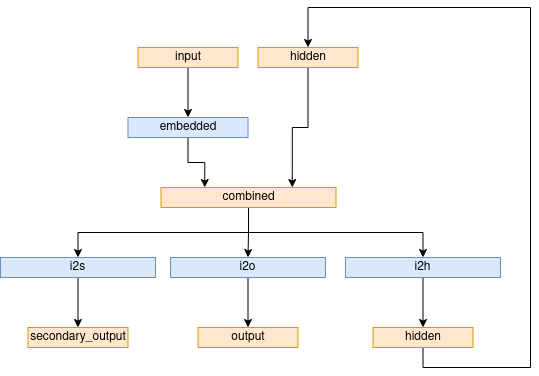
\includegraphics[width=0.5\linewidth]{img/modele_with_secondary.png}
    \caption{Modèle RNN avec tâche secondaire}

    \label{fig:modele_rnn_with_secondary}
\end{figure}

\section{Fonctionnalités développées}
Ainsi que mentionné précédemment, nous avons élaboré un modèle de classification des émotions, en ajoutant une tâche secondaire dédiée à la détection de la négation. Nous avons aussi réalisé une analyse de la distribution des mots, le filtrage des termes rares, et l'identification des mots porteurs de sens à l'aide de la méthode TF-IDF. \\
Parallèlement, nous avons conduit une étude sur l'impact de la taille de la couche d'embedding dans deux scénarios distincts : l'un avec un grand nombre de paramètres et l'autre avec un nombre limité de paramètres. De plus, nous avons évalué l'influence de l'attribution de poids en fonction de la fréquence d'apparition des émotions dans notre ensemble d'entraînement. Cette démarche visait à équilibrer l'apprentissage des émotions très fréquentes par rapport à celles moins fréquentes.

\section{Résultats}

Notre modèle par défaut est entrainé sur 20 époques avec des taille de lots de 8, des tailles de couches (embedding et hidden) de 100, un taux d'apprentissage de $10^{-4}$, un poids de tâche secondaire de 0.1 et les fonctionnalités de filtrage (TF-IDF) des mots rares et de poids d'équilibrage des émotions (\textit{emotions\_weight}).
\\\\
INSERER TABLEAU RESULTATS ET GRAPHIQUES

\end{document}